\documentclass[letterpaper,10pt]{article}

\usepackage{titling}
\usepackage{listings}
\usepackage{url}
\usepackage{setspace}
\usepackage{subfig}
\usepackage{sectsty}
\usepackage{pdfpages}
\usepackage{colortbl}
\usepackage{multirow}
\usepackage{relsize}
\usepackage{amsmath}
\usepackage{fancyvrb}
\usepackage{amsmath,amssymb,amsthm,graphicx,xspace}
\usepackage[titlenotnumbered,noend,noline]{algorithm2e}
\usepackage[compact]{titlesec}
\usepackage[default]{droidserif}
\usepackage[T1]{fontenc}
\usepackage{tikz}
\usetikzlibrary{arrows,automata,shapes,trees,matrix,chains,scopes,positioning,calc}
\tikzstyle{block} = [rectangle, draw, fill=blue!20, 
    text width=2.5em, text centered, rounded corners, minimum height=2em]
\tikzstyle{bw} = [rectangle, draw, fill=blue!20, 
    text width=4em, text centered, rounded corners, minimum height=2em]

\definecolor{namerow}{cmyk}{.40,.40,.40,.40}
\definecolor{namecol}{cmyk}{.40,.40,.40,.40}

\let\LaTeXtitle\title
\renewcommand{\title}[1]{\LaTeXtitle{\textsf{#1}}}


\newcommand{\handout}[5]{
  \noindent
  \begin{center}
  \framebox{
    \vbox{
      \hbox to 5.78in { {\bf ECE155: Engineering Design with Embedded Systems } \hfill #2 }
      \vspace{4mm}
      \hbox to 5.78in { {\Large \hfill #4  \hfill} }
      \vspace{2mm}
      \hbox to 5.78in { {\em #3 \hfill} }
    }
  }
  \end{center}
  \vspace*{4mm}
}

\newcommand{\lecture}[3]{\handout{#1}{#2}{#3}{Lecture #1}}
\newcommand{\tuple}[1]{\ensuremath{\left\langle #1 \right\rangle}\xspace}

\addtolength{\oddsidemargin}{-1.000in}
\addtolength{\evensidemargin}{-0.500in}
\addtolength{\textwidth}{2.0in}
\addtolength{\topmargin}{-1.000in}
\addtolength{\textheight}{1.75in}
\addtolength{\parskip}{\baselineskip}
\setlength{\parindent}{0in}
\renewcommand{\baselinestretch}{1.5}
\newcommand{\term}{Spring 2014}

\singlespace



\begin{document}

\lecture{ 32 --- Software Architecture Patterns}{\term}{Jeff Zarnett}

\section*{Software Architecture}
A software architecture pattern is a general, re-usable solution to how to structure (``architect'') a piece of software. At a very high level, nearly all pieces of software contain three major elements: 

\begin{enumerate}
	\item Logic -- the software does some work,
	\item Data -- it stores and/or retrieves some data somehow, and
	\item User Interface -- it presents information to and accepts information and/or commands from the user or users.
\end{enumerate}


It is rare if not impossible to find an application in the business world that is purely built using one architecture. Many programs contain elements that make use of more than one architectural style, depending on the nature of the program. Different architectural patterns are appropriate for different applications, or even different parts of the same application. The architectures that are chosen are also not always consistently followed. This is normal; real world software complexity will require some deviation from the pattern. 

\paragraph{Motivation.} Our motivation for using architecture patterns is similar to the motivation for following a software lifecycle model or development management process. In school assignments, with the possible exception of the Fourth Year Design Project, when working on software you can probably get away without choosing a structure (you will likely end up with the Monolith situation, described below). This works okay when you're dealing with a small project over a short period of time, but to work on anything significantly bigger or more complex, you will need to make a meaningful choice about how the software should be structured; otherwise you might just end up creating a \textit{bug farm} (a piece of code where many bugs are found) or creating unnecessary work for yourself later on when you try to bring some order to the chaos.

\subsection*{The Monolith}
A monolithic application is one in which all elements are combined into a single, self-contained program. There are no defined modules, no components, and no clear lines between different parts of the application. The logic, user interface, and data are all mixed together. In the early days of software development, a lot of mainframe applications were written like this. Probably all of the code you have written in an academic context so far has been monolithic (but this may change if/when you take a class like Distributed Systems). However, as programs got larger and more complex, the complexity spirals out of control and becomes unmaintainable. Hopefully any program you have worked on during a co-op term has had a different structure.

The monolith structure is simple to understand and often faster to write than a more structured program. However, it is difficult to maintain. If the internals of a class or part of the system are available for other classes to use, sooner or later some class is going to start using them and depending on them. Parts that are tightly interconnected may be hard if not impossible to upgrade or change. Changes in one area may have unexpected consequences in another area. Although the monolith structure has many disadvantages, it is not necessarily the ``wrong'' choice. There are many successful commercial applications that use this structure, such as Microsoft Word.


\subsection*{Client-Server Architecture}
In the client-server architecture, there are two roles in the system, the client and the server, and they communicate with a request-response message pattern. The client sends a request to the server, and the server sends a response back. To make this work, the client and server must be able to understand one another and therefore agree on a communication protocol. The client-server architecture is very common in computer networks. E-mail, the Web, and banking are all systems making use of the client-server architecture.

\begin{center}
	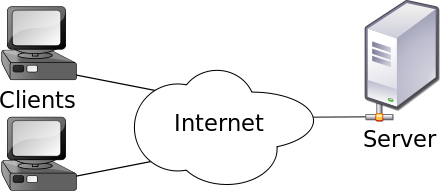
\includegraphics[width=0.4\textwidth]{images/Client-server-model.png}
	
	\texttt{\small
 http://en.wikipedia.org/wiki/File:Client-server-model.svg}
\end{center}

There is a clear line dividing the server from the client, and the roles of each party are defined. Most often, the logic and data elements reside on the server, and the client handles the user interface. The client does not need to concern itself with how the server formats its response. Often, the client and server programs run on different physical machines, but it is not a requirement. 

In the case of the web, when you request \texttt{www.google.com} with your browser, the browser needs no knowledge of how the server at Google composes its answer. Similarly, the server at Google does not care about how the request is generated or how the browser draws the web page on the screen after receiving the response. 

As a historical note, at one time, a lot of computing was done using the client-server architecture. When personal computers were still expensive and mainframes were common, the computer sitting on a worker's desk was sometimes a ``thin client'' or ``dumb terminal'': it had very little processing power of its own and simply sent work to the server to be executed and provided some based on the server's response. For example, when compiling code, a user might have entered it on the terminal on her desk and then submitted a request (sometimes called a ``batch job'') for the mainframe to take that code, compile it, and return the result. Starting in the 1980s, the prices of PCs decreased and their power increased dramatically, making it more efficient to buy more powerful PCs and have them do more of the work. Now when we compile code it's almost always done on the local device (although in co-op you might have encountered a build server that builds official versions of the software for testing and release). 

It is typically possible to replace either the client or the server, as long as the communication protocol is unchanged. You can, sticking with the web example, open \texttt{www.google.com} with Chrome or Firefox and this makes no difference to the server, since the request and response are the same. This is a big improvement over the monolith structure because it separates concerns. If the server is centralized, however, a server crash might prevent the whole system from functioning. Aside: some people may attempt to cause a server crash with the explicit intent of denying all other users access to the server, but we'll talk about security later on in the term.


\subsection*{Three-Tier Architecture}

Three-Tier architecture is similar to the client-server architecture in that it is comprised of multiple separate, interacting parts. However, in this model, the user interface, the logic, and the data each reside in their own component of the system; these are most often on separate systems (such as the client's PC, a logic server, and a database server), but as with the client-server architecture, that is not mandatory~\cite{threeTier}. 


Each of the separate tiers can be changed out or modified without affecting the tiers below or above; if the presentation tier is upgraded to run on Android phones as well as as a PC application, this has no impact on the logic or data tiers of the application. Similarly, you might swap the data tier out, moving from mySQL to Oracle, and similarly the client and logic tiers would be unaffected.

In the following image, the tiers are shown and explained; note that what we call the user interface is called the ``presentation tier'' below.

\begin{center}
	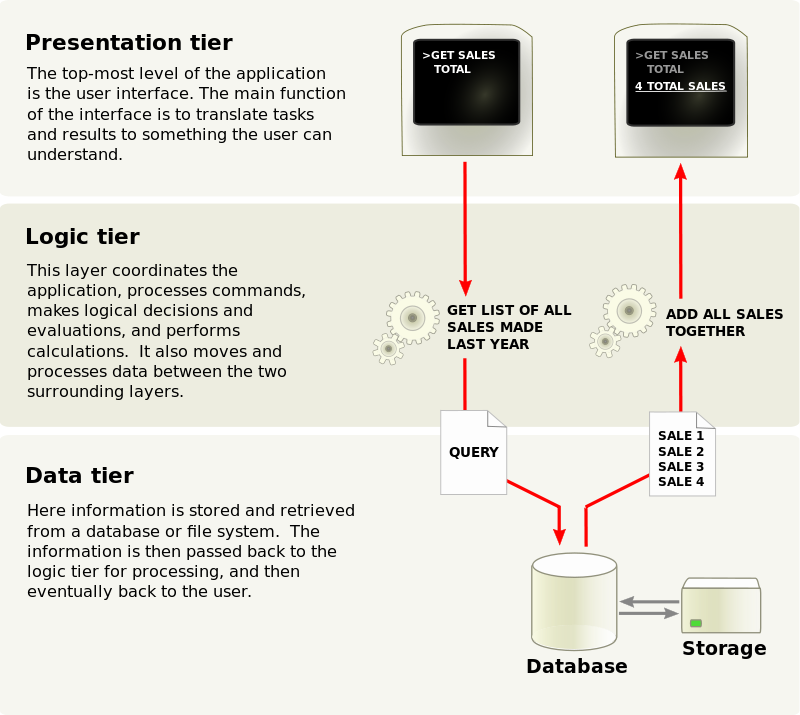
\includegraphics[width=0.5\textwidth]{images/threetier.png}
	
	\texttt{\small
 http://en.wikipedia.org/wiki/File:Overview\_of\_a\_three-tier\_application\_vectorVersion.svg}
\end{center}


Note that it is possible for the logic tier to be further subdivided, resulting in ``n-tier architecture''.

\paragraph{Overlap with Client-Server} As previously mentioned, in a client-server architecture, the most common split is for the user interface (presentation tier) to be on the client and the logic and data tiers to take place on the server (or servers). However, the line between client and server may not be identical to the line between the presentation and logic tiers. In fact, it is common to have the client capable of some logic on its own (perhaps validating input, or pre-processing a file to be uploaded), so the dividing line between client and server could be anywhere. However, the presentation tier does not communicate directly with the data tier; it is always moderated through the logic tier.

It is also noteworthy that the client-server kind of interaction could exist between any two \textit{adjacent} tiers of the system. In addition to the obvious case of the presentation tier being a client to the logic tier's server, from the perspective of the data tier, the data tier is the server responding to requests from a client, in this case the logic tier.

Re-visiting the Google example from earlier, when you search Google for something, you can envision the interaction not just as client-server, but as a three tier architecture. Your browser sends to the server your search request (``xkcd telescope names''). The server analyzes this request and queries their database for matches on these search terms. The database returns the results, which the logic tier takes and formats into a webpage. The logic tier sends the answer back to your browser (presentation tier), and the browser draws the page on the screen.

\subsection*{Model-View-Controller Architecture}

Model-View-Controller (MVC) is a very common pattern that divides the software application into three different parts, the model, view, and controller, and the pattern also defines the interactions between the three parts \cite{posa}. Imagine a piece of data, a \texttt{Contact} object that has contact information for a person or business, such as name, phone number, postal address, et cetera. 


The \textbf{Model} holds a reference to the \texttt{Contact}, as well as the business logic and actions (methods/functions). It is the responsibility of the model to notify the view(s) and controller(s) if the object has been updated, so the other parts of the system know to update (and in a later lecture we will address the subject of events). Only the model has direct access to the object being worked on; the other elements of the system must go through the model to make changes or view the information.

The \textbf{View} is any representation of the \texttt{Contact} data. There can be multiple views of the same data, such as a fancy looking e-card on the screen, or a simple plain-text version for printing. The view requests from the model what data it needs to display.

The \textbf{Controller} accepts input and converts that into commands for the model or view. Commands sent to the model are used to manipulate the state of the object in question; commands sent to the view are used to change the view (for example, scrolling down or maximizing a window).

\paragraph{Example.} Suppose the user wants to make a change, such as setting the phone number equal to null. The user clicks on a button labelled ``Clear Phone Number''. This input is taken by the controller and turned into a command that the model can understand, such as \texttt{setPhoneNumber(null)}. The model executes this command and it notifies the view that the data has been updated. The view is then redrawn to show the phone number field of the \texttt{Contact} is blank. The user then sees the change on screen.
This sequence of interactions is described in general terms in the following diagram:

\begin{center}
	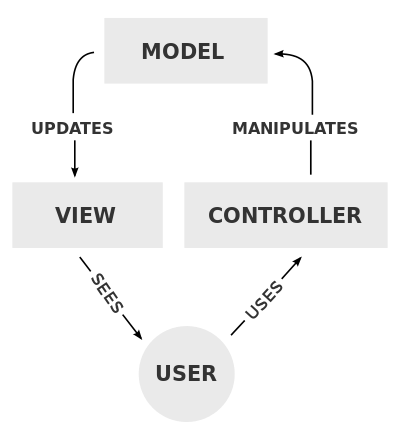
\includegraphics[width=0.35\textwidth]{images/mvc.png}
	
	\texttt{\small http://en.wikipedia.org/wiki/File:MVC-Process.svg}
\end{center}

MVC is considered good programming practice because it separates the logic code from the code that is used to display information to the user. This makes it much easier to have different views available, such as having a full screen (desktop) version of an application and a small screen (mobile) version. Modularity also means that certain elements can be changed (most often the view) without requiring any changes to the others. Of course, this does not mean that these elements never need to be updated: if a new field is added to the \texttt{Contact}, like Twitter Account, it would be sensible to add that field to the UI and add the methods to get, set, and clear this field.

\paragraph{Overlap with Client-Server.} The MVC architecture is compatible with the client-server architecture; that is, it is possible to use both of them in the same system. In a client-server system, the client might call up a record from the server and then use MVC for the user to manipulate it, with one of the model actions being to save the changes (send them back to the server for storage). In a thin-client system, the client might only have the view and controller, while the server has the model; in other situations all three will be on the client side.

\paragraph{Overlap with Three-Tier.} The MVC architecture is also compatible with the three-tier architecture. The view and controller belong in the presentation tier, while the model is in the logic tier. The MVC, client-server, and n-tier architectures can then obviously exist in the same complex system. One way this might happen is the client has the view and controller (presentation tier), the server has the model (logic tier), and the objects represented, such as the \texttt{Contact} described earlier, is stored in the data tier (also on the server side).


\subsection*{Modular Architecture} 
As defined so far, the client and server (or tiers) might themselves be described as being monolithic in that they are opaque and self-contained. However, even in a system that uses clients and servers, one or both of those might be too complex to build as a monolith and instead should be built in a modular way. The name comes from the word module, and as expected the final software product will be comprised of a number of modules which interact in some way. A module, sometimes called a component, contains a related set of methods/functions or data.  The modular architecture is also sometimes called ``Component-Based Software Engineering'' and is generally considered a good thing. 

Consider as an example a travel loyalty program where users can collect points and redeem them for rewards. This system could be comprised of a number of different components (modules), each responsible for a specific area, such as billing the credit card.

\begin{center}
	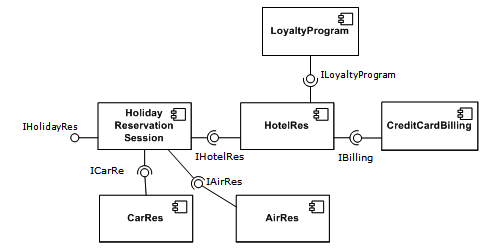
\includegraphics{images/cbse.png}
	
	\texttt{\small
http://en.wikipedia.org/wiki/File:Component-based-Software-Engineering-example2.gif}
\end{center}

\newpage

As you may have guessed, the existence of the distinct boxes enclosing modules suggests that different modules may be replaced or upgraded independently of the others. This is often desirable. If the loyalty program moves to a new airline, they can replace the air reservation module (AirRes in the diagram) without changing the other parts of the system.

Under ideal circumstances, components can also be re-used elsewhere in the system or in another system. If the company running the loyalty program decided to expand its business by opening up a rewards shop, where you could buy items online. If the credit card billing module is implemented well, that component can be re-used, without changes, in the online store system. 



\bibliographystyle{alpha}
\bibliography{155}


\end{document}